\chapter{Progettazione e sviluppo}\label{chapter:progettazionesviluppo}
In questo capitolo saranno esposti gli approcci teorici e pratici per lo sviluppo del progetto.

\section{Containerizzazione con Docker}\label{sec:ContDocker}
Sulla base di quanto spiegato precedentemente, per quanto riguarda la creazione e l'utilizzo delle applicazioni cloud – native, sono stati introdotti i cosiddetti \emph{Orchestratori di container}, che sono utilizzati per racchiudere e allo stesso tempo isolare, una o più applicazioni nel loro ambiente di esecuzione, con i relativi file necessari.\\
In altre parole, i container possono essere visti come delle Virtual Machine (infatti possiedono molte delle caratteristiche) che però non eseguono un sistema operativo nella sua interezza, ma solo l'applicazione di cui si necessita ed eventuali altri servizi coinvolti nel ciclo di vita di questa.\\
I container risultano essere comodi e affidabili per l'utilizzo in tutti i momenti della creazione di un nuovo software, dallo sviluppo al test, fino alla fase finale di produzione.\\
Altri due vantaggi che si possono ottenere dall'utilizzo dei container, così come per le Virtual Machine, riguardano la sicurezza e la scalabilità.\\
La prima è conseguenza del fatto che, come detto sopra, si riesce ad isolare l'applicazione in esecuzione in un determinato container e quindi, se dovessero esserci problemi (nella maggior parte dei casi possono verificarsi problemi inevitabili), questi non potrebbero intaccare in nessun modo altri container e quindi il funzionamento di altre applicazioni.\\
La scalabilità è garantita dal fatto che un container può essere creato, gestito e modificato in base alle necessità, non esistono \emph{container standard}, ognuno viene adattato per lo scopo da raggiungere.\\

\begin{figure}[ht]
    \centering
    \resizebox{0.8\textwidth}{!}{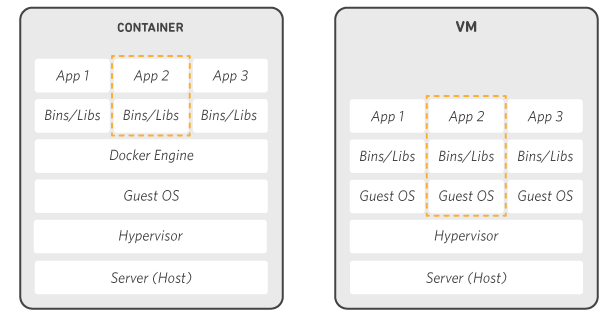
\includegraphics{img/containervsvm.png}}
    \caption{Container e Virtual Machine a confronto}
    \label{fig:one}
\end{figure}

Docker è un software open source per la creazione e la gestione di container.\\
L'utilizzo di Docker si basa sulle \emph{Docker images} che possono essere utilizzate per:
\begin{itemize}
\item Template per la creazione di container
\item Starting point per un container
\item Eseguire codice all'interno di un container 
\end{itemize}

Le \emph{Docker images} possono essere prelevate da Docker Hub, la raccolta ufficiale di immagini messe a disposizione per gli utenti, oppure si può scrivere un file di testo, il \texttt{Dockerfile}, per racchiudere tutti i comandi per assemblare un'immagine durante la fase di buil


\section{Introduzione ai microservizi}\label{sec:microserviziintro}
Prima di introdurre il concetto di architettura a microservizi è bene introdurre il concetto di architettura monolitica.\\
Un'architettura monolitica è una metodologia di sviluppo secondo la quale tutti i processi coinvolti sono strettamente legati tra di loro e sono erogati 
come un singolo servizio.\\
Questa tipologia di approccio porta ad avere sistemi nei quali modificare le funzionalità diventa più complesso, in quanto si deve agire sull'intero sistema e non 
solo sulle parti effettivamente interessate.\\
Inoltre, utilizzare un'architettura monolitica porta a correre dei rischi per quanto riguarda la disponibilità dell'applicazione, in quanto anche se solo uno dei 
processi coinvolti avesse un malfunzionamento, questo si propagherebbe nell'intera applicazione.\\ \\
Per quanto riguarda le architetture a microservizi, queste sono diametralmente opposte alle architetture monolitiche.\\
Nelle architetture a microservizi l'obiettivo è quello di scomporre l'applicazione da realizzare nelle sue funzioni (\emph{servizi}) di base.\\
Ogni servizio può essere compilato e distribuito in modo indipendente; quindi i singoli servizi possono funzionare o non funzionare senza compromettere gli altri.\\
Utilizzare i microservizi significa riuscire a gestire criticità inevitabili, poter sfruttare la scalabilità dinamica e semplificare l'integrazione 
di nuove caratteristiche. \cite{RedHatMicroservices}, \cite{Amazon}\\

\begin{figure}[ht]
	\centering
	\resizebox{1.0\textwidth}{!}{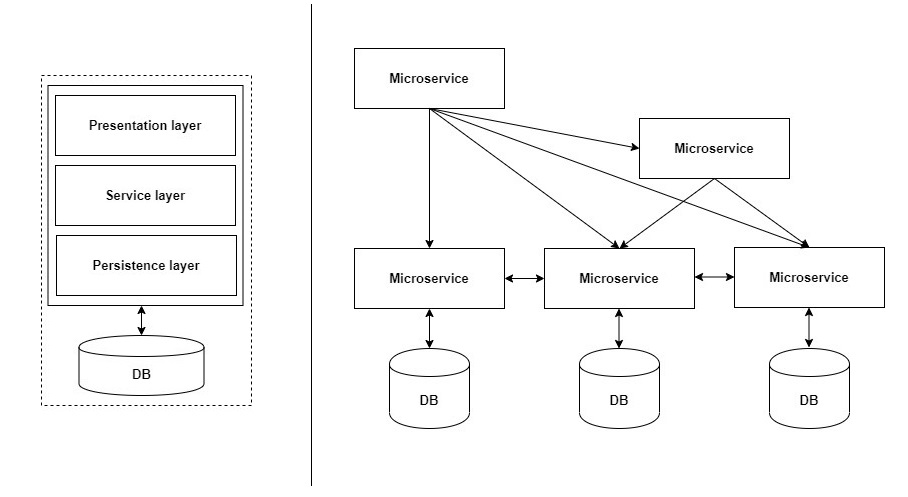
\includegraphics{img/monovsmicro}}
	\caption{Architettura monolitica e architettura a microservizi a confronto}
	\label{fig:one}
\end{figure}

Oggi i container Linux permettono di eseguire più parti di un'applicazione in modo indipendente con un controllo superiore sui singoli componenti.\\
I microservizi containerizzati rappresentano la base delle applicazioni cloud native. \cite{RedHatDocker}\\ \\
Di seguito sono elencati alcuni dei vantaggi di un'architettura a microservizi:

\begin{itemize}
	\item \textbf{Agilità}\\ Essendo ogni applicazione suddivisa in servizi di base, i team di sviluppo agiscono in contesti ridotti, semplificando il lavoro e riducendo i tempi del ciclo di sviluppo.
	\item \textbf{Scalabilità}\\Lavorare con un microservizio consente di scalare in modo indipendente per rispondere alla richiesta di un determinato servizio.\\ In questo modo è possibile misurare il carico di lavoro di un singolo servizio e adattarlo di conseguenza; il che può portare a dei vantaggi anche in termini economici per il mantenimento dell'applicazione. 
	\item \textbf{Semplicità di distribuzione}\\ I microservizi supportano l'approccio \emph{CI/CD} (Continuous Integration/Continuous Delivery), così da semplificare l'integrazione e il testing di nuove funzionalità avendo comunque la possibilità di effettuare un rollback in caso di problemi.
	\item \textbf{Codice riutilizzabile}\\ Uno dei vantaggi del suddividere un'applicazione in servizi è la possibilità di poter riutilizzare codici di servizi già esistenti per altre applicazioni.
	\item \textbf{Resilienza}\\ Avendo un'applicazione a servizi indipendenti si aumenta la resilienza in caso di errori.\\ Si possono gestire completamente gli errori di un servizio isolando la funzionalità senza bloccare l'intera applicazione.
\end{itemize}

\section{Il microservizio \texttt{CheckEmail}}\label{sec:architetturamicroservizio}
Il microservizio realizzato verifica l'avvenuto acquisto di un modulo applicativo da parte di un utente identificato, ai fini del microservizio, tramite un indirizzo e-mail.\\
Lo scopo principale del microservizio è quello di ricevere una richiesta \texttt{HTTP} con all'interno del body un indirizzo e-mail.\\
Una volta estratto l'indirizzo e-mail il microservizio effettua una \emph{query} all'interno del Database per controllare che l'indirizzo sia presente nella tabella degli utenti abilitati all'utilizzo di un determinato servizio.\\
In base al risultato della query il microservizio restituisce un codice \texttt{HTTP} come risposta alla richiesta.\\
\newline
La tipologia di richieste descritte sono effettuate tramite il metodo \textbf{\texttt{GET}} di \texttt{HTTP}, quindi vengono richiesti dei dati dal server.\\
\newpage
I codici che possono essere restituiti sono:\\
\begin{table}[ht]
	\centering
	\resizebox{1.0\linewidth}{!}{
		\begin{tabularx}{\linewidth}{|>{\centering\arraybackslash}m{3cm}|>{\centering\arraybackslash}m{4cm}|>{\centering\arraybackslash}m{5cm}|}
			\hhline{|-|-|-|}
			\textbf{Codice HTTP} & \textbf{Significato} & \textbf{Descrizione}\\
			\hhline{|-|-|-|}
			200 & OK & Il microservizio ha risposto correttamente e l'utente è autorizzato a procedere. \\
			\hhline{|-|-|-|}
			402 & PAYMENT REQUIRED & Il microservizio ha risposto correttamente ma l'utente non è autorizzato a procedere.\\
			\hhline{|-|-|-|}
			500 & INTERNAL SERVER ERROR & Messaggio di errore generico, non si è potuto raggiungere il microservizio.\\
			\hhline{|-|-|-|}
			503 & SERVICE UNAVAILABLE & Server non disponibile, non si è potuto raggiungere il microservizio. \\
			\hhline{|-|-|-|}
		\end{tabularx}
	}
	\vspace*{6mm}
	\caption{Codici HTTP restituiti dal microservizio}
	\label{tab:httpcode}
\end{table}

\begin{figure}[ht]
	\centering
	\resizebox{0.9\textwidth}{!}{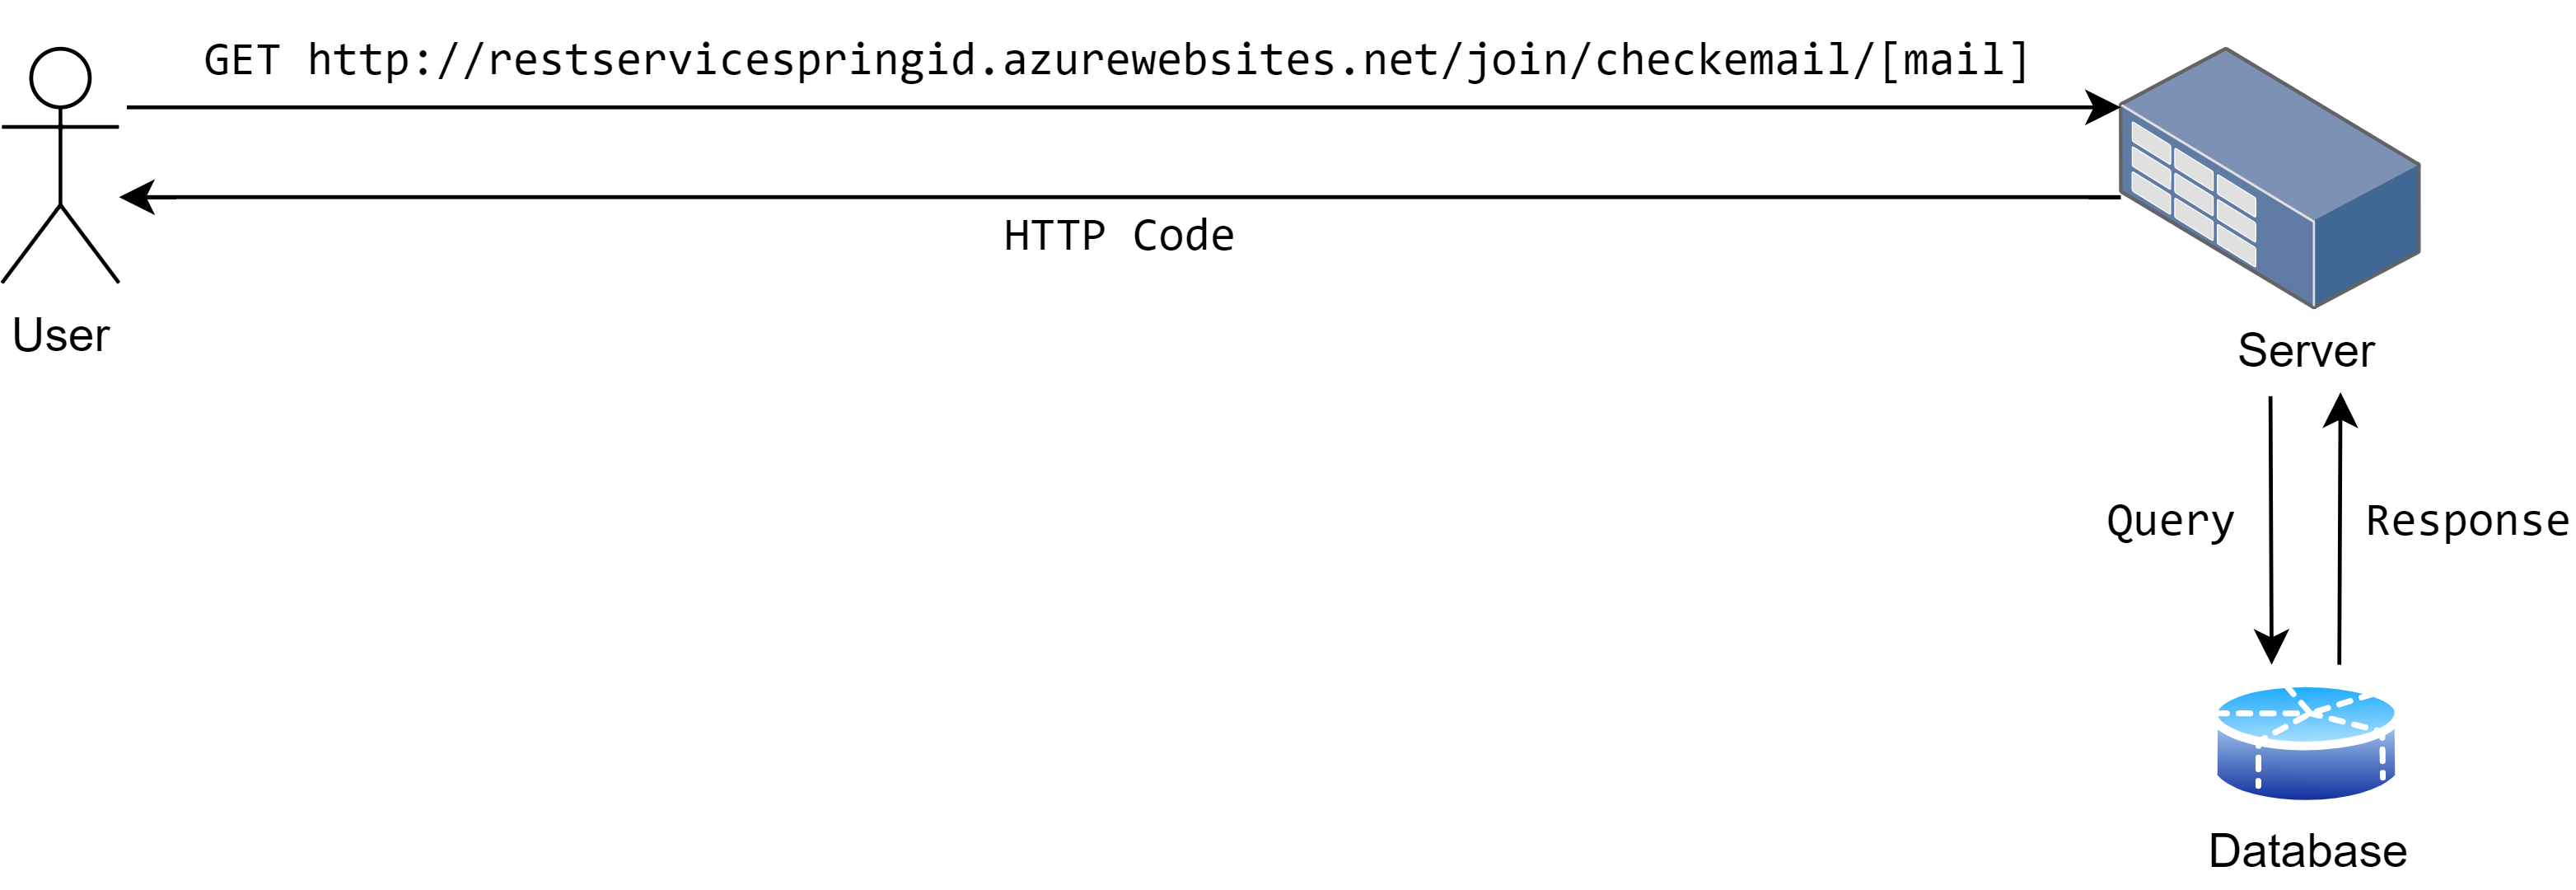
\includegraphics{img/comunicazionemicroservizio}}
	\caption{Schema di comunicazione Utente - microservizio}
	\label{fig:one}
\end{figure}
\newpage
\subsection{Sviluppo Database}\label{sec:sviluppodatabase}
Per sviluppare ed utilizzare il microservizio si è resa necessaria la creazione del Database PostgreSQL per la memorizzazione dei dati degli utenti.\\
È bene premettere che il Database è stato volutamente creato nella maniera più semplice e facilmente manutenibile, dato che durante lo sviluppo questo doveva 
servire solo per scopi di testing.\\
Il Database è composto da due tabelle:
\begin{itemize}
		\item \textbf{\texttt{users}}\\ Contiene le informazioni di tutti gli utenti abilitati ad accedere ad un determinato servizio.
		\item \textbf{\texttt{email}}\\ Contiene gli indirizzi e-mail di tutti gli utenti della piattaforma, quindi non è garantito che tutti avranno accesso a tutti i servizi.
\end{itemize}
\begin{figure}[ht]
	\centering
	\resizebox{0.3\textwidth}{!}{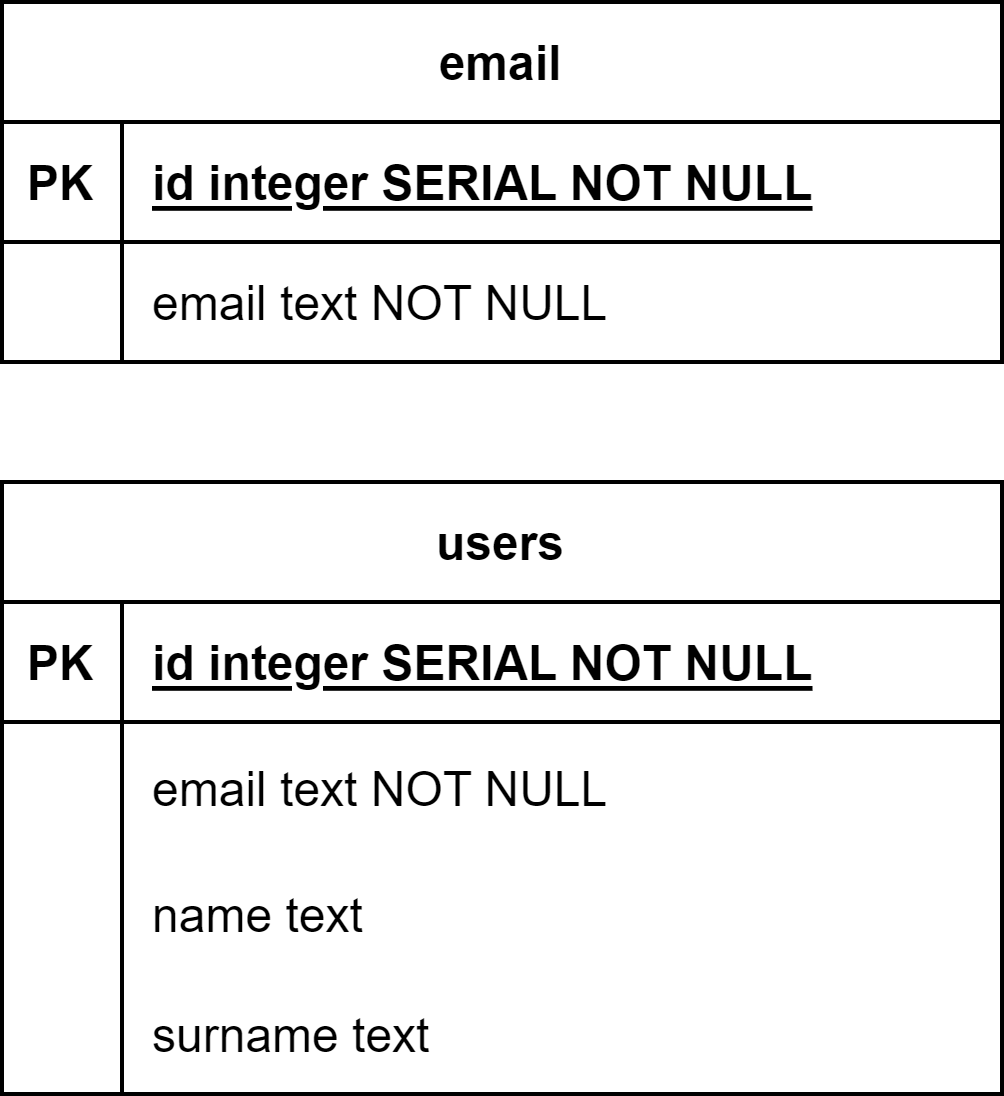
\includegraphics{img/dbtables-drawio}}
	\caption{Modello Entità Relazione del Database}
	\label{fig:one}
\end{figure}

\begin{figure}[ht]
	\centering
	\resizebox{0.7\textwidth}{!}{\includegraphics{img/emaildb_e}}
	\caption{Contenuto delle tabelle visualizzato dalla shell di PostgreSQL}
	\label{fig:one}
\end{figure}
\newpage
\subsection{Sviluppo Microservizio}\label{sec:sviluppomicroservizio}
Per lo sviluppo del microservizio, come accennato in precedenza, è stato deciso di utilizzare il linguaggio di programmazione Java e il framework Spring.\\
Il progetto è stato realizzato utilizzando l'IDE Eclipse ed è composto da cinque \emph{package}.\\
Descrizione dei package:
\begin{itemize}
	\item \textbf{\texttt{com.aesys.valeriodesiati.mail}}\\ Contiene la classe principale del microservizio.
	\item \textbf{\texttt{com.aesys.valeriodesiati.mail.model}}\\ Contiene le classi relative alle entità all'interno del Database.\\
	\emph{Spring Boot JPA} consente la creazione di entità in un Database a partire da una normale classe Java tramite l'aggiunta di annotazioni fornite dal framework.
	\item \textbf{\texttt{com.aesys.valeriodesiati.mail.repository}}\\ Contiene le interfacce relative alle entità del Database che ereditano l'interfaccia 
	\mintinline{java}{JpaRepository<T,ID>}.\\ Tale interfaccia contiene le API per tutte le operazioni CRUD di base.\\ CRUD (Create Read Update Delete) è un acronimo 
	che indica le quattro operazioni fondamentali per creare un'applicazione che abbia uno storage persistente.
	\item \textbf{\texttt{com.aesys.valeriodesiati.mail.controller}}\\ Contiene le classi \emph{Controller} del microservizio, ovvero le classi annotate con 
	\mintinline{java}{@RestController}.\\ In Spring una classe annotata come \emph{Controller} è una classe che sarà utilizzata come handler di richieste web.
	\item \textbf{\texttt{com.aesys.valeriodesiati.mail.exception}}\\ Contiene le classi per la definizione di \emph{custom exception}.\\ L'implementazione 
	di tali classi si è resa necessaria per poter comprendere meglio gli errori in fase di sviluppo e di debug.\\
\end{itemize}

\newpage
Di seguito i diagrammi UML dei package principali del microservizio:
\begin{figure}[H]
	\centering
	\resizebox{0.5\textwidth}{!}{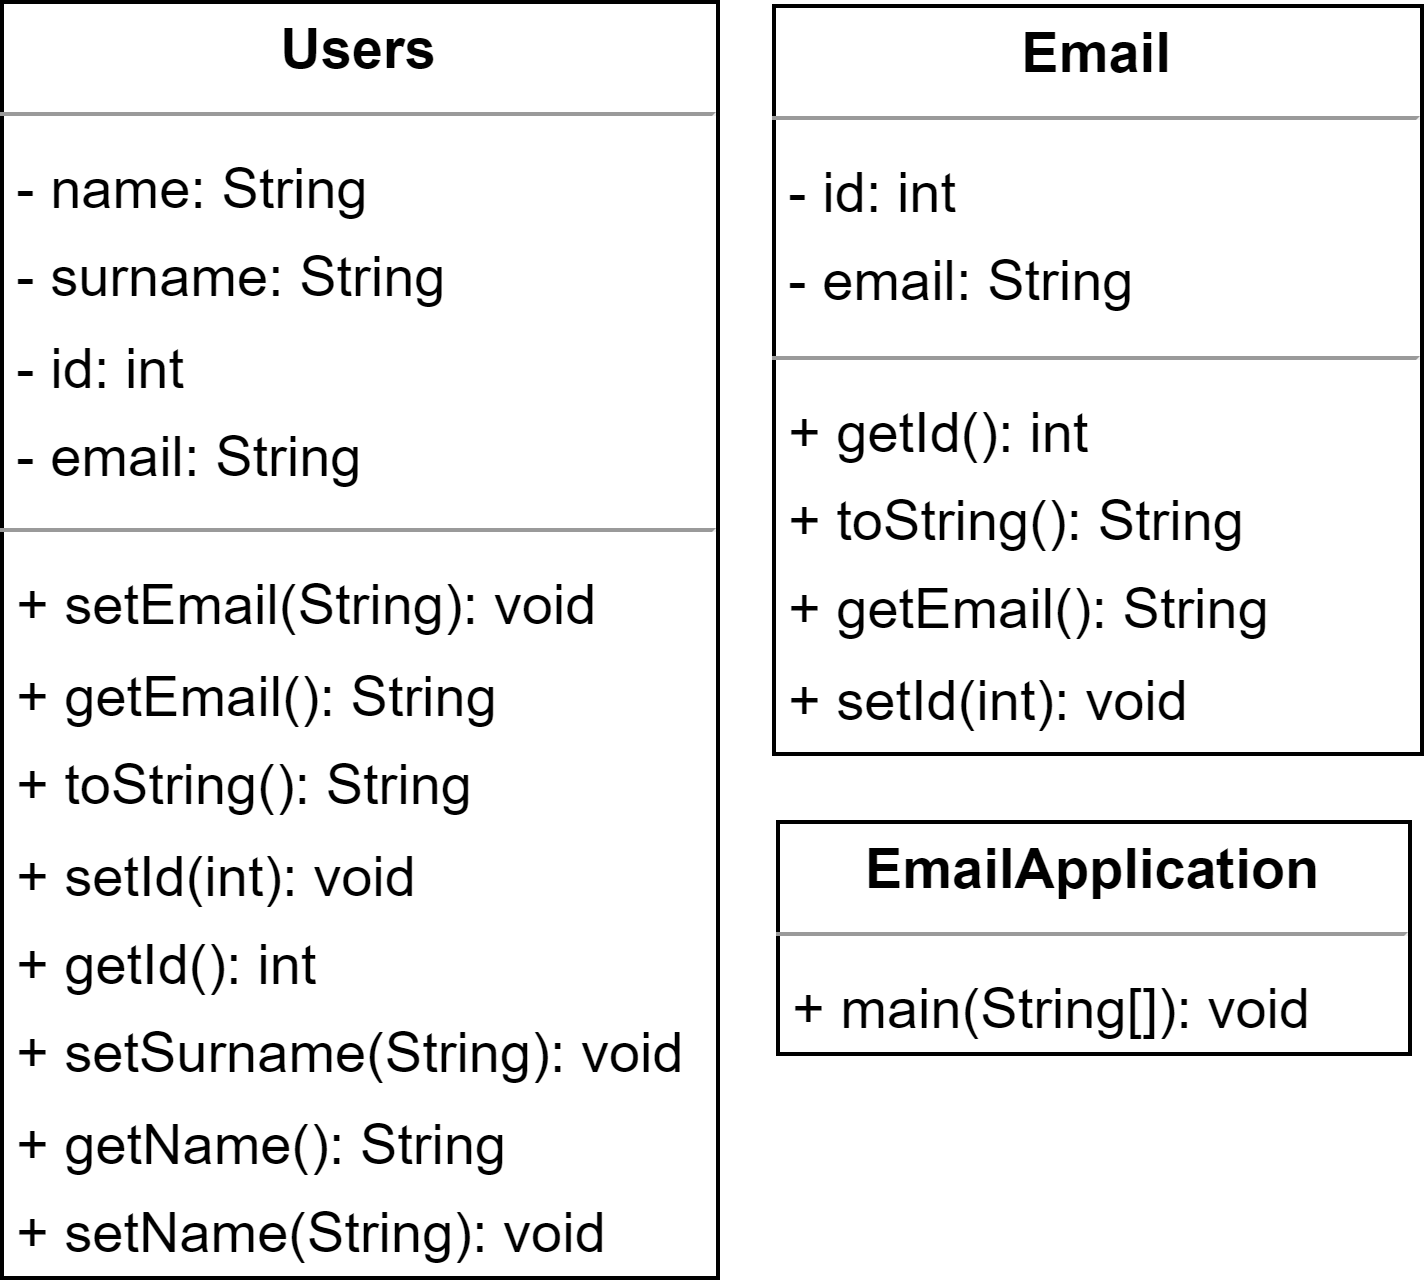
\includegraphics{img/classi}}
	\caption{Diagramma UML delle classi principali del progetto}
	\label{fig:umlclass}
\end{figure}

\begin{figure}[H]
	\centering
	\resizebox{0.7\textwidth}{!}{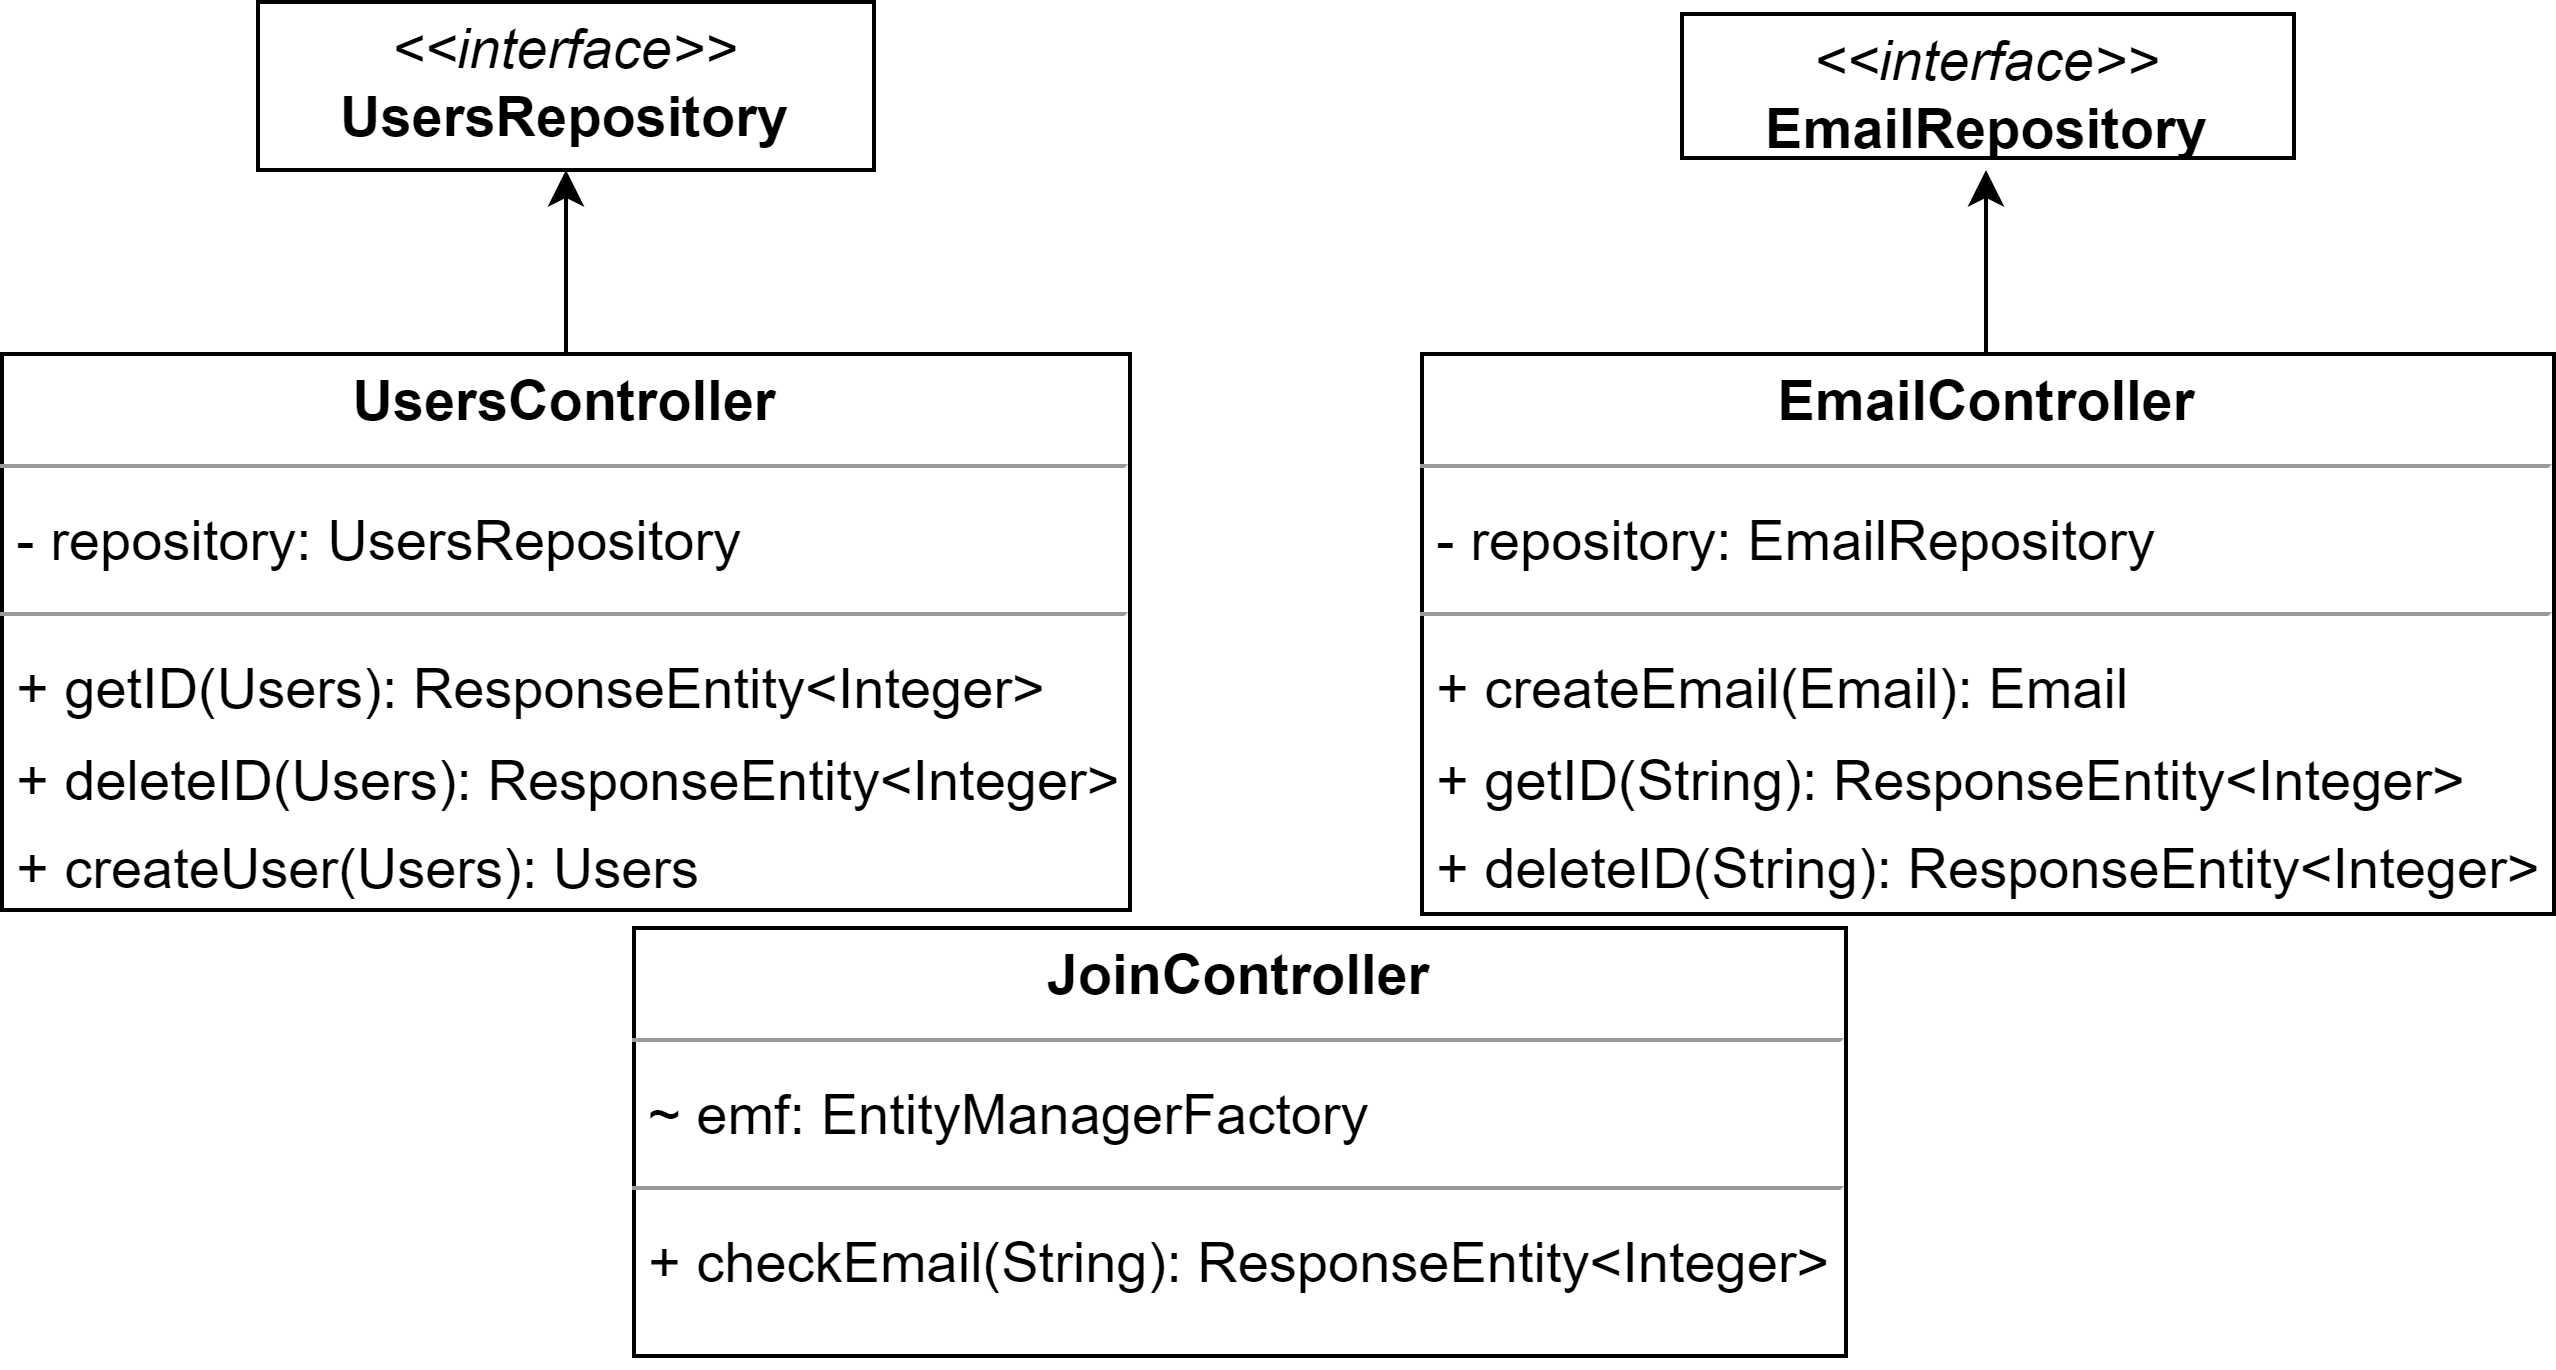
\includegraphics{img/controller}}
	\caption{Diagramma UML delle classi \emph{controller} del progetto}
	\label{fig:umlcontroller}
\end{figure}

\begin{figure}[H]
	\centering
	\resizebox{0.7\textwidth}{!}{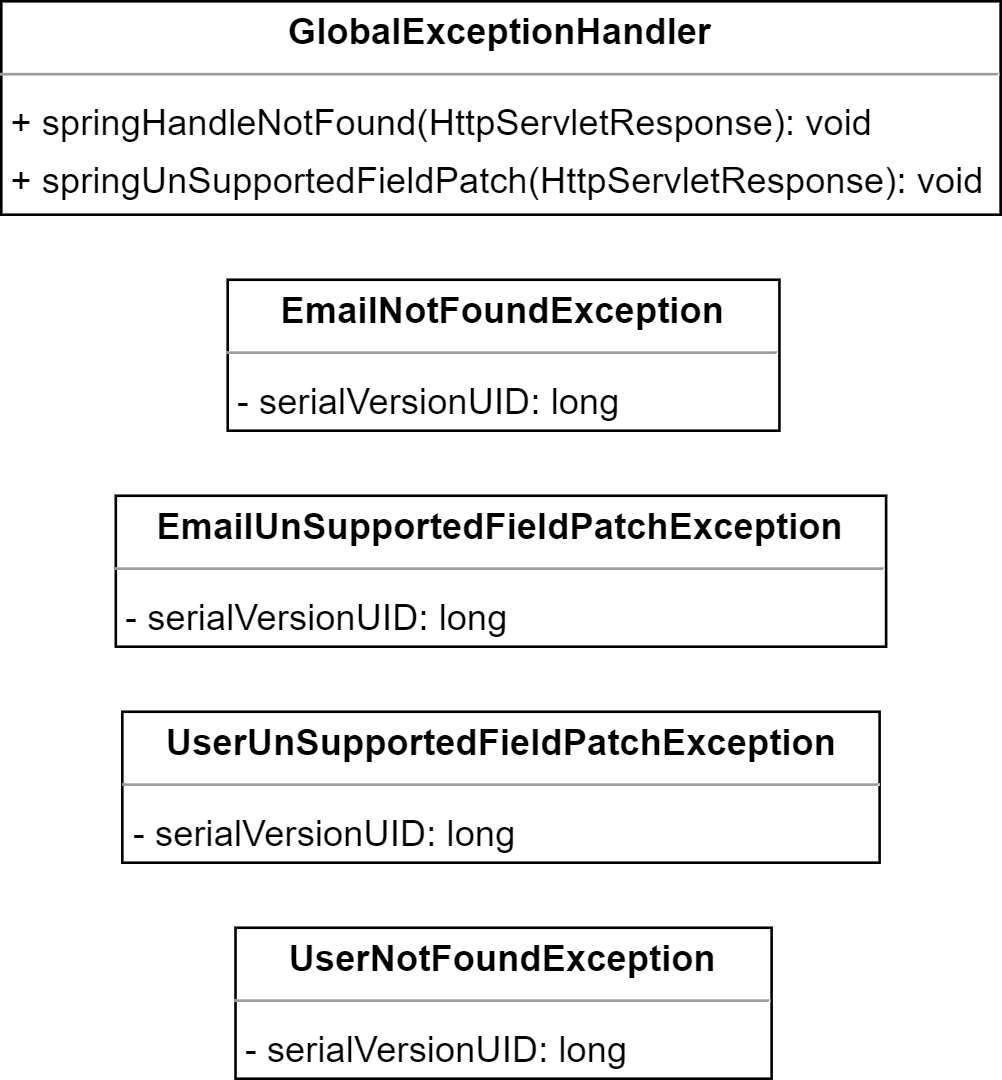
\includegraphics{img/exception}}
	\caption{Diagramma UML delle \emph{custom exception} del progetto}
	\label{fig:umlexception}
\end{figure}
\newpage

\subsubsection{\texttt{EmailApplication.java}}
\begin{algorithm}
\centering
\begin{minted}[fontsize=\scriptsize, xleftmargin=20pt,linenos]{java}
package com.aesys.valeriodesiati.mail;

import org.springframework.boot.SpringApplication;
import org.springframework.boot.autoconfigure.SpringBootApplication;

@SpringBootApplication
public class EmailApplication {
    
    public static void main(String[] args) {
        SpringApplication.run(EmailApplication.class, args);
    }

}
\end{minted}
\caption{Classe \emph{mail} del progetto}\label{alg:emailapplication}
\end{algorithm}

La classe principale del progetto è composta da un solo comando, che si occupa di avviare l'applicazione.\\
Il metodo \mintinline{java}{run()} è il metodo principale di Spring Framework, serve ad avviare tutti i processi necessari per l'esecuzione dell'applicazione.\\
La prima cosa che è possibile notare è che il metodo \mintinline{java}{run()} prende come parametri il file bytecode della classe stessa ed eventuali argomenti.\\
Nello specifico, il metodo \mintinline{java}{run()}:
\begin{itemize}
\item Legge le configurazioni.
\item Avvia l'Application Context, un gestore per tutte le classi coinvolte nell'esecuzione dell'applicazione.
\item Scansiona il Path dell'intero progetto, per trovare e organizzare tutte le classi annotate con \mintinline{java}{@Controller}, \mintinline{java}{@RestController}, \mintinline{java}{@Entity } ecc.
\item Se richiesto, avvia Tomcat Server per il deploy e l'avvio dell'applicazione.
\end{itemize}
\newpage
\subsubsection{\texttt{Users.java}}
\begin{algorithm}[H]
\centering
\begin{minted}[fontsize=\scriptsize, breaklines, xleftmargin=20pt,linenos]{java}
package com.aesys.valeriodesiati.mail.model;
//imports..
@Entity
@Table (name="users")
public class Users {

    @Id
    @GeneratedValue(strategy=GenerationType.IDENTITY)
    private int id;
    @Column(name = "email", nullable = false)
    private String email;
    @Column(name = "name")
    private String name;
    @Column(name = "surname")
    private String surname;

    public Users(int id, String email, String name, String surname) {
        this.id = id;
        this.email = email;
        this.name = name;
        this.surname = surname;
    }

    //setters, getters, toString()...
}
\end{minted}
\caption{Classe \mintinline{java}{@Entity} Users.java}\label{alg:usersjava}
\end{algorithm}

È bene precisare da subito che il comportamento delle classi \texttt{Users.java} e \texttt{Email.java} è molto simile, 
in quanto entrambe annotate come \mintinline{java}{@Entity}.\\
Una classe annotata come \mintinline{java}{@Entity} indica che questa servirà per la creazione di una tabella all'interno del Database specificato, 
utilizzando come campi gli attributi della classe.\\
È possibile notare come la classe \texttt{Users.java} sia una classe molto “standard” per quanto riguarda la creazione di oggetti di tipo \texttt{Users}, 
le uniche aggiunte solo le annotazioni Spring, come ad esempio:
\begin{itemize}
\item \mintinline{java}{@Id} e \mintinline{java}{@GeneratedValue()} per definire l'attributo come \emph{id} autogenerato.
\item \mintinline{java}{@Column()} per definire il nome di un campo (colonna) della tabella ed eventuali altre proprietà.
\end{itemize}
\newpage
\subsubsection{\texttt{JoinController.java}}
\begin{algorithm}[H]
\centering
\begin{minted}[fontsize=\scriptsize, breaklines, xleftmargin=20pt,linenos]{java}
package com.aesys.valeriodesiati.mail.controller;
//imports..
@RestController
public class JoinController {
    
    @Autowired
    EntityManagerFactory emf;
    
    @Transactional
    @GetMapping("/join/checkemail/{mail}")
    public ResponseEntity<Integer> checkEmail(@PathVariable("mail") String mail) {
        
        EntityManager em = emf.createEntityManager();
        em.getTransaction().begin();
        String result = null;
        
        try {
            result = (String) em.createQuery("SELECT u.email
                                                  FROM Users u, Email e
                                                  WHERE u.email = e.email 
                                                  AND u.email = :email")
                                                  .setParameter("email", mail)
                                                  .getSingleResult();
        }
        catch(NoResultException | NullPointerException e) {
            return ResponseEntity.status(HttpStatus.PAYMENT_REQUIRED).body(402);
        }
        
        if(result == null)
            return ResponseEntity.status(HttpStatus.PAYMENT_REQUIRED).body(402);
        else
            return ResponseEntity.status(HttpStatus.OK).body(200);
            
    }
}

\end{minted}
\caption{Classe \mintinline{java}{@RestController} JoinController.java}\label{alg:joincontrollerjava}
\end{algorithm}

Si tratta della classe che svolge il compito principale del microservizio, ovvero controllare che l'indirizzo mail specificato si trovi nella 
tabella \texttt{email}, ma anche nella tabella \texttt{users}, proprio a certificare che l'indirizzo dato sia abilitato a procedere.\\
La classe è annotata come \mintinline{java}{@RestController}, utilizzato per la gestione di richieste \texttt{HTTP}.\\
I metodi che possono essere utilizzati con questa tipologia di Controller sono \mintinline{java}{@RequestMapping}, \mintinline{java}{@GetMapping}, 
\mintinline{java}{@PostMapping}, \mintinline{java}{@PutMapping},\\ \mintinline{java}{@DeleteMapping} ecc., si devono sempre specificare l'URL e il tipo di richiesta da gestire.
In un'architettura REST le risorse sono rappresentate in modo da essere compatibili con le operazioni CRUD (Create, Read, Update, Delete).\\
Successivamente troviamo un \mintinline{java}{EntityManager} utilizzato l'interazione con il Database ed è parte del modulo Spring Data JPA.\\
Consente la creazione, la modifica, la rimozione e il caricamento di entità (tabelle) nel Database. \\ \\
Andando ad analizzarne più a fondo le specifiche è possibile notare, in testa al metodo, l'annotazione\\ \\
\centerline{\mintinline{java}{@GetMapping("/join/checkemail/{mail}")}} \\ \\
tramite la quale diventa possibile intercettare delle richieste \texttt{HTTP GET} effettuate in un determinato percorso. Il parametro \mintinline{java}{{mail}} può essere
utilizzato all'interno della funzione.\\
Si prosegue con la creazione e l'esecuzione della query, che effettua un'operazione di join tra le tabelle \texttt{Users} e \texttt{Email}, andando a 
svolgere le operazioni descritte più in alto.\\
Il tutto è svolto all'interno di un blocco \mintinline{java}{try{ } catch(Exception){ }} al fine di prevenire comportamenti anomali: se viene lanciata l'eccezione\\
\mintinline{java}{NoResultException} o \mintinline{java}{NullPointerException}, si ritorna il codice \texttt{HTTP 402 Payment Required}.
Se si termina l'esecuzione della query senza eccezioni e la variabile \mintinline{java}{result} non è impostata a \mintinline{java}{null}, si ritorna il codice \texttt{HTTP 200 OK}.

\subsubsection{\texttt{application.properties}}
\begin{algorithm}
\centering
\begin{minted}[fontsize=\scriptsize, breaklines, xleftmargin=20pt,linenos]{sh}
	spring.jpa.properties.hibernate.jdbc.lob.non_contextual_creation=true
	spring.datasource.url=
		jdbc:postgresql://postgresqlkong.postgres.database.azure.com:5432
				/fattdb?ssl=true&sslmode=require
	spring.datasource.username=*****
	spring.datasource.password=*****
\end{minted}
\caption{File di configurazione \texttt{application.properties}}\label{alg:applicationproperties}
\end{algorithm}
Il file \texttt{application.properties} è utilizzato per definire proprietà aggiuntive dell'applicazione come nel nostro caso, il Database.\\
È possibile vedere come siano definiti tutti i parametri per la connessione al Database PostgreSQL, all'interno del quale saranno 
create le tabelle ed effettuate le query.

\newpage

\section{Introduzione a Kong Gateway}\label{sec:kongprog}
Come accennato nel paragrafo \ref{sec:kongintro}, \emph{Kong Gateway} è un API gateway cloud-native che fornisce l'opportunità di configurare \emph{services} e \emph{routes} e, oltre a questi, anche \emph{plugin} e \emph{consumer}.
\subsection{Service}\label{sec:kongservice}
Un \emph{service} in Kong Gateway è un'astrazione di tutti i servizi upstream custom che si aggiungono alla configurazione. Con \emph{servizio upstream custom} si intende un microservizio custom che prende dati dalla richiesta inoltrata al gateway e ne restituisce altri al gateway stesso, che si occuperà di comunicarli al client.\\
Solitamente ad ogni \emph{service} è associata una o più \emph{routes}. \cite{Kong}\\

\subsection{Route}\label{sec:kongroute}
Una \emph{route} è una regola definita per indirizzare correttamente le richieste del client.\\
L'associazione di una (o più) route ad un servizio consente di realizzare un meccanismo di routing molto potente, dato che è possibile configurare
 nel dettaglio il percorso che si vuole realizzare (con i relativi protocolli da utilizzare, livello di sicurezza ecc.). \cite{Kong}

\subsection{Consumer}\label{sec:kongconsumer}
Un \emph{consumer} in Kong Gateway può essere inteso come un utente di uno specifico servizio e può essere identificato tramite un \texttt{id} univoco. \cite{Kong}

\subsection{Plugin}\label{sec:kongplugin}
Un \emph{plugin} è un'entità che sarà eseguita durante tutto il ciclo di vita di una richiesta o risposta HTTP/S (HyperText Trasfer Protocol / Secure).\\
È il modo in cui Kong Gateway fornisce la possibilità di ottenere funzionalità aggiuntive per un \emph{service} o una \emph{route}.\\
I plugin configurabili possono essere sia proprietari (attivabili da Kong Manager) sia custom. Per la realizzazione di un plugin custom si ha la possibilità 
di scegliere tra vari linguaggi di programmazione per lo sviluppo quali Go, Python, JavaScript e Lua (linguaggio utilizzato per lo sviluppo 
del plugin custom utilizzato nel progetto). \cite{Kong}

\section{Architettura del plugin \texttt{checkemail}}\label{sec:architetturaplugin}
Un plugin in Lua per Kong Gateway si compone principalmente di due file:

\begin{itemize}
	\item \textbf{\texttt{handler.lua}}\\ Questo file contiene tutta la logica del plugin, devono essere implementate tutte le funzioni coinvolte nel ciclo richiesta/risposta.
	\item \textbf{\texttt{schema.lua}}\\ Racchiude tutte le configurazioni addizionali, se necessarie, come ad esempio coppie chiave/valore o altre impostazioni per modificare il comportamento del plugin.
\end{itemize}

Il funzionamento e l'utilizzo di questi file sarà approfondito nel paragrafo successivo e nel paragrafo \ref{sec:kongconf}.

\subsection{Sviluppo}\label{sec:sviluppoplugin}
Come detto in precedenza la logica del plugin è interamente contenuta nel file \texttt{handler.lua}.\\ 
È richiesto il seguente comportamento dal plugin:

\begin{enumerate}
	\item Analizzare il token ricevuto.
	\item Parse del token.
	\item Inviare una richiesta \texttt{HTTP} al microservizio \texttt{CheckEmail}.
	\item Ottenere risposta dal microservizio e inoltrarla al Gateway.
\end{enumerate}

Il primo punto è realizzato dalla funzione \mintinline{lua}{SplitToken(token)}, che analizza il token \texttt{JWT} ricevuto e lo suddivide nelle tre parti di cui è composto: Header, Body e Signature.\\
La funzione restituisce un array contenente le tre componenti del token.

\begin{algorithm}
\centering
\begin{minted}[fontsize=\scriptsize, xleftmargin=20pt, linenos]{lua}
	local function SplitToken(token)
		local segments = {}
		for str in string.gmatch(token, "([^\\.]+)") do
			table.insert(segments, str)
		end
		return segments
	end
\end{minted}
\caption{Suddivisione token JWT}\label{alg:splittoken}
\end{algorithm}

Successivamente si procede con il parse del token, mediante la funzione \mintinline{lua}{ParseToken(token)} che inizia chiamando la funzione \mintinline{lua}{SplitToken(token)}
per ottenere l'array delle parti, per poi proseguire applicando una decodifica ad ogni parte controllando anche l'eventuale presenza di errori.\\
La funzione può restituire tre o quattro risultati: nel caso in cui non ci siano stati errori vengono restituite solo le tre componenti del token decodificate, altrimenti 
vengono restituiti quattro risultati, i primi tre impostati a \mintinline{lua}{null} (rappresentano i campi del token) e il quarto come stringa con un messaggio di errore.\\
Da notare come tutte le parti vengano prima suddivise e poi decodificate anche se il dato ricercato (l'indirizzo mail) si trova solo nel Body, questo per favorire e semplificare 
la ricerca di eventuali componenti del token corrotte.

\begin{algorithm}
\centering
\begin{minted}[fontsize=\scriptsize, xleftmargin=20pt, linenos]{lua}
	local function ParseToken(token)
		local segments = SplitToken(token)
		if #segments ~= 3 then
			return nil, nil, nil, "Invalid token"
		end

		local header, err = cjson_safe.decode(basexx.from_url64(segments[1]))
		if err then
			return nil, nil, nil, "Invalid header"
		end

		local body, err = cjson_safe.decode(basexx.from_url64(segments[2]))
		if err then
			return nil, nil, nil, "Invalid body"
		end

		local sig, err = basexx.from_url64(segments[3])
		if err then
			return nil, nil, nil, "Invalid signature"
		end

		return header, body, sig
	end
\end{minted}
\caption{Parse token JWT}\label{alg:parsetoken}
\end{algorithm}
\newpage
Il ciclo di funzionamento del plugin termina quindi con l'estrazione dell'indirizzo mail dal token decodificato e l'inoltro della richiesta \texttt{HTTP} al microservizio \texttt{CheckEmail}.\\
Il microservizio è raggiungibile al link\\ \texttt{ http://restservice-springid.azurewebsites.net/join/checkemail/}, \\
unendo al link l'indirizzo mail che si desidera controllare, come riportato di seguito.\\
\begin{algorithm}
\centering
\begin{minted}[fontsize=\scriptsize, xleftmargin=20pt, linenos]{lua}
    local body, code, headers, status = 
			http.request("http://restservice-springid.azurewebsites.net
				      /join/checkemail/"..bodyTok.email)
\end{minted}
\caption{Inoltro richiesta \texttt{HTTP} dal plugin}\label{alg:pluginhttprequest }
\end{algorithm}

L'ultimo controllo che si effettua è quello sul codice di ritorno \texttt{HTTP} ricevuto dal microservizio, che viene quindi inoltrato da Kong Gateway all'utente.

\begin{algorithm}
\centering
\begin{minted}[fontsize=\scriptsize, xleftmargin=20pt, linenos]{lua}
    if code == 200 then
        return kong.response.exit(200, "Success")
    end

    if code == 402 then
        return kong.response.error(402, "Payment Required")
    end

	--response codes 500 and 503...
\end{minted}
\caption{Inoltro risposta dal plugin a Kong Gateway}\label{alg:plugingatewayresponse}
\end{algorithm}

\section{Configurazione Kong Gateway}\label{sec:kongconf}
Kong Gateway è stato containerizzato tramite Docker utilizzando l'immagine ufficiale presente su Docker Hub.\\
Il container è stato reso raggiungibile tramite una macchina virtuale su Azure con immagine Debian.\\
Sono state create delle pipeline CI/CD per automatizzare i processi di containerizzazione e di installazione del plugin.\\
La pipeline è azionata automaticamente dai cambiamenti nella repository principale del progetto e si occupa di far eseguire, all'interno della macchina virtuale, 
uno script per l'aggiornamento dei \emph{services}, \emph{routes}, \emph{consumers}.
\newpage
Il gateway può essere configurato in modi diversi:
\begin{itemize}
\item Interfaccia grafica di Kong Manager, disponibile collegandosi da browser alla porta 8002 del container.
\item Tramite file JSON contenenti le informazioni necessarie che saranno aggiunte al file di configurazione principale (\texttt{kong.conf}), inoltrati con delle richieste \texttt{HTTP POST} verso il container in esecuzione.
\end{itemize}
\ \\
Come detto in precedenza, gli aspetti configurabili sono:
\begin{itemize}
	\item\emph{Services}
	\item\emph{Routes}
	\item\emph{Consumers}
	\item\emph{Plugin}
\end{itemize}

Ognuno con un file JSON di configurazione dedicato.\\
I plugin custom, come quello realizzato, non necessitano di un file di configurazione dedicato, è sufficiente copiare i file relativi nella directory\\
\texttt{/usr/local/share/lua/5.1/kong/plugins/nome\_plugin/} del container.\\

Tutta la configurazione è effettuata tramite lo script bash \texttt{addplugin} che ha i seguenti compiti:
\begin{itemize}
\item Avviare il container.
\item Copiare al suo interno i file relativi ai plugin custom.
\item Riavviare il container (per consentire la lettura dei file dei plugin caricati)
\item Eseguire il comando \mintinline{bash}{curl} per tutti i file JSON presenti relativi a tutte le altre configurazioni necessarie.
\end{itemize}
\newpage
Di seguito alcune righe dello script di configurazione:

\begin{algorithm}
\centering
\begin{minted}[fontsize=\scriptsize, xleftmargin=20pt, linenos]{sh}
    sudo docker exec -it --user root $container rm -rf 
				/usr/local/share/lua/5.1/kong/plugins/$dir
    sudo docker exec -it --user root $container mkdir
				/usr/local/share/lua/5.1/kong/plugins/$dir
    sudo docker cp . $container:/usr/local/share/lua/5.1/kong/plugins/$dir/
    curl -s -X POST -H "Content-Type: application/json"
	-d @./config/checkemail/services.json
	http://checkemail.westeurope.cloudapp.azure.com:8001/services > /dev/null
\end{minted}
\caption{Script per la configurazione di Kong Gateway}\label{alg:container_config}
\end{algorithm}

